\documentclass[a4paper]{article}
\usepackage[top=.5in,textheight=10in]{geometry}
\usepackage{amsmath,amssymb,amsfonts,amsthm,mathtools,enumitem}
\usepackage{booktabs}
\usepackage{geometry}
\usepackage{fancyhdr}
\usepackage{graphicx}

\pagestyle{fancy}
\fancyhf{}
\rhead{Notes Title}
\lhead{\leftmark}
\cfoot{\thepage }   


\geometry{paper=a4paper, margin=100pt, includeheadfoot}

\theoremstyle{definition}
\newtheorem*{defi}{Definition}
\newtheorem*{eg}{Example}
\newtheorem*{prop}{Proposition}
\newtheorem*{thm}{Theorem}


\title{Precalculus Notes}
\author{Duncan F. Bandojo \\ 11-Newton}
\begin{document}
\maketitle

\tableofcontents
\setcounter{section}{-1}
\section{Introduction}
Welcome to Precalculus Notes

\section{Conic Sections }
\begin{defi}[Conic Section]
    A \emph{conic} is the curve obtained as the intersection of a plane, called
    the cutting plane, with the surface of a double right circular cone.
\end{defi}
\begin{defi}[Circle]
    The \emph{circle} is obtained when the cutting plane is perpendicular to the
    axis of symmetry of the cone and parallel to the plane of the generating
    \emph{circle} of the cone.
\end{defi}
\begin{defi}[Parabola]
    If the cutting plane is parallel to exactly one generating line of the cone,
    then the conic is unbounded and is called a \emph{parabola}
\end{defi}
\begin{defi}[Ellipse]
    \emph{Ellipses} arise when the intersection of the cone and plane is a
    closed curve. The plane that intersects the curve is neither parallel or
    perpendicular to the axis of symmetry.
\end{defi}
\begin{defi}[Hyperbola]
     The plane that intersects the cone is parallel to the axis of symmetry of
     the cone, cutting both halves of the cone, producing two separate unbounded
     curves.
\end{defi}

\subsection{Circle}
\begin{defi}[Circle]
    A circle with center $(h, k)$ and radius $r > 0$ is the set of all points
     $(x,y)$ in the plane whose distance to $(h,k)$ is $r$.
     \begin{equation*}
          r=\sqrt{(x-h)^2+(y-k)^2}
     \end{equation*}
\end{defi}
By squaring both sides of this equation, we get an equivalent equation (since $r
> 0$) which gives us the

\begin{figure}[h]
     \centering
     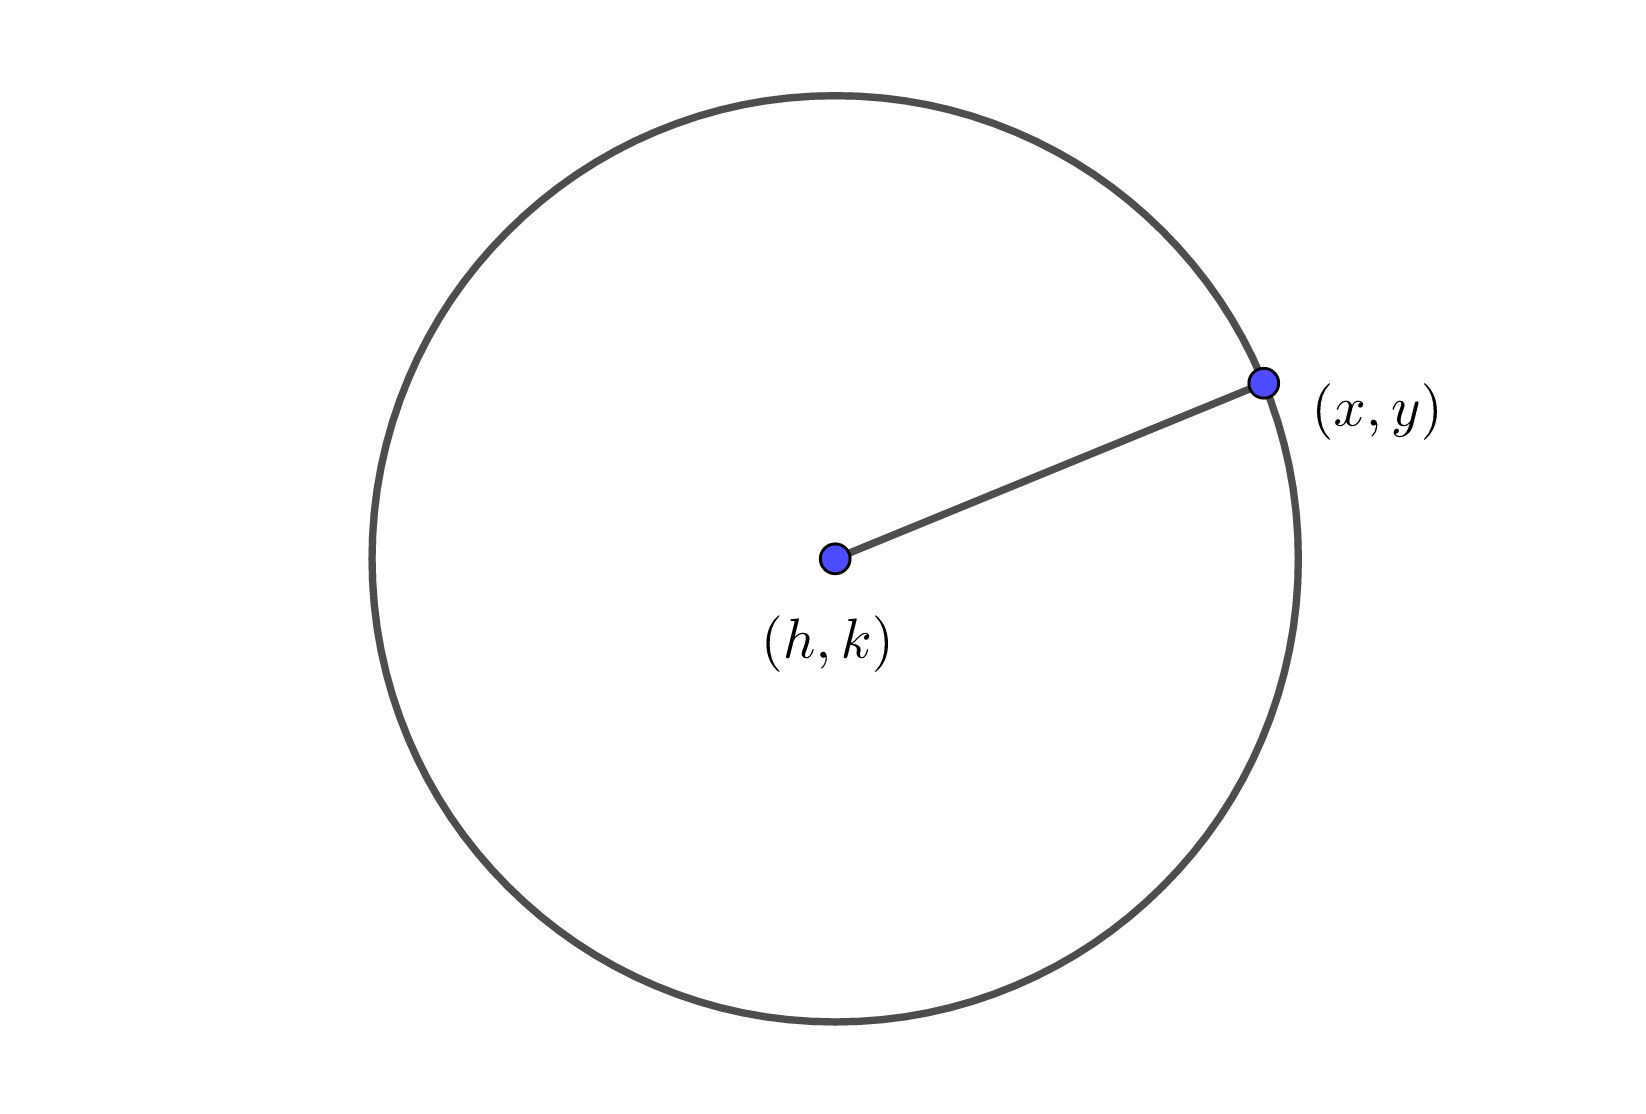
\includegraphics[scale = .8]{circle1.png}
\end{figure}

\begin{defi}[Standard Equation of a Circle]
     The equation of a circle with center $(h,k)$ and radius $r>0$ is 
     \begin{equation*}
        (x-h)^2+(y-k)^2 = r^2
     \end{equation*} 
\end{defi}
\begin{defi}[General Equation of a Circle]
     \begin{equation*}
          x^2+y^2+Dx+Ey+F=0
     \end{equation*}
     For some constants $D, E,$ and $F$.
\end{defi}
There are $3$ cases that might happen to the radius $r$.    
\begin{itemize}
     \item $r^2 > 0$ $\rightarrow$ Circle
     \item $r^2 = 0$ $\rightarrow$ Degenerate Circle or Point Circle
     \item $r^2 < 0$ $\rightarrow$ $\emptyset$
\end{itemize}
\begin{defi}[Distance from Point to Line]
     Distance from a point $(x_1,y_1)$ to a line $Ax+By+C=0$.
     \begin{equation*}
          d = \dfrac{\sqrt{Ax_1+By_1+C}}{\sqrt{A^2+B^2}}
     \end{equation*}
\end{defi}

\subsection{Parabola}

\begin{defi}[Parabola]
    Let $F$ be a point in the plane and $\ell$ be a line not containing $F$. A
     \emph{parabola} is the set of all points equidistant from $F$ and $\ell$.
     The point $F$ is called the \emph{focus} of the parabola and the line
     $\ell$ is called the \emph{directrix} of the \emph{parabola}.
\end{defi}
\begin{defi}[Standard Equation of a Vertical Parabola]
     The equation with Vertex $V:(h,k)$ and focal length $c$ is
     \begin{equation*}
          (x-h)^2 = \pm4c(y-k)
     \end{equation*}
     Opening either upward or downward.
\end{defi}

\begin{figure}[h]
     \centering
     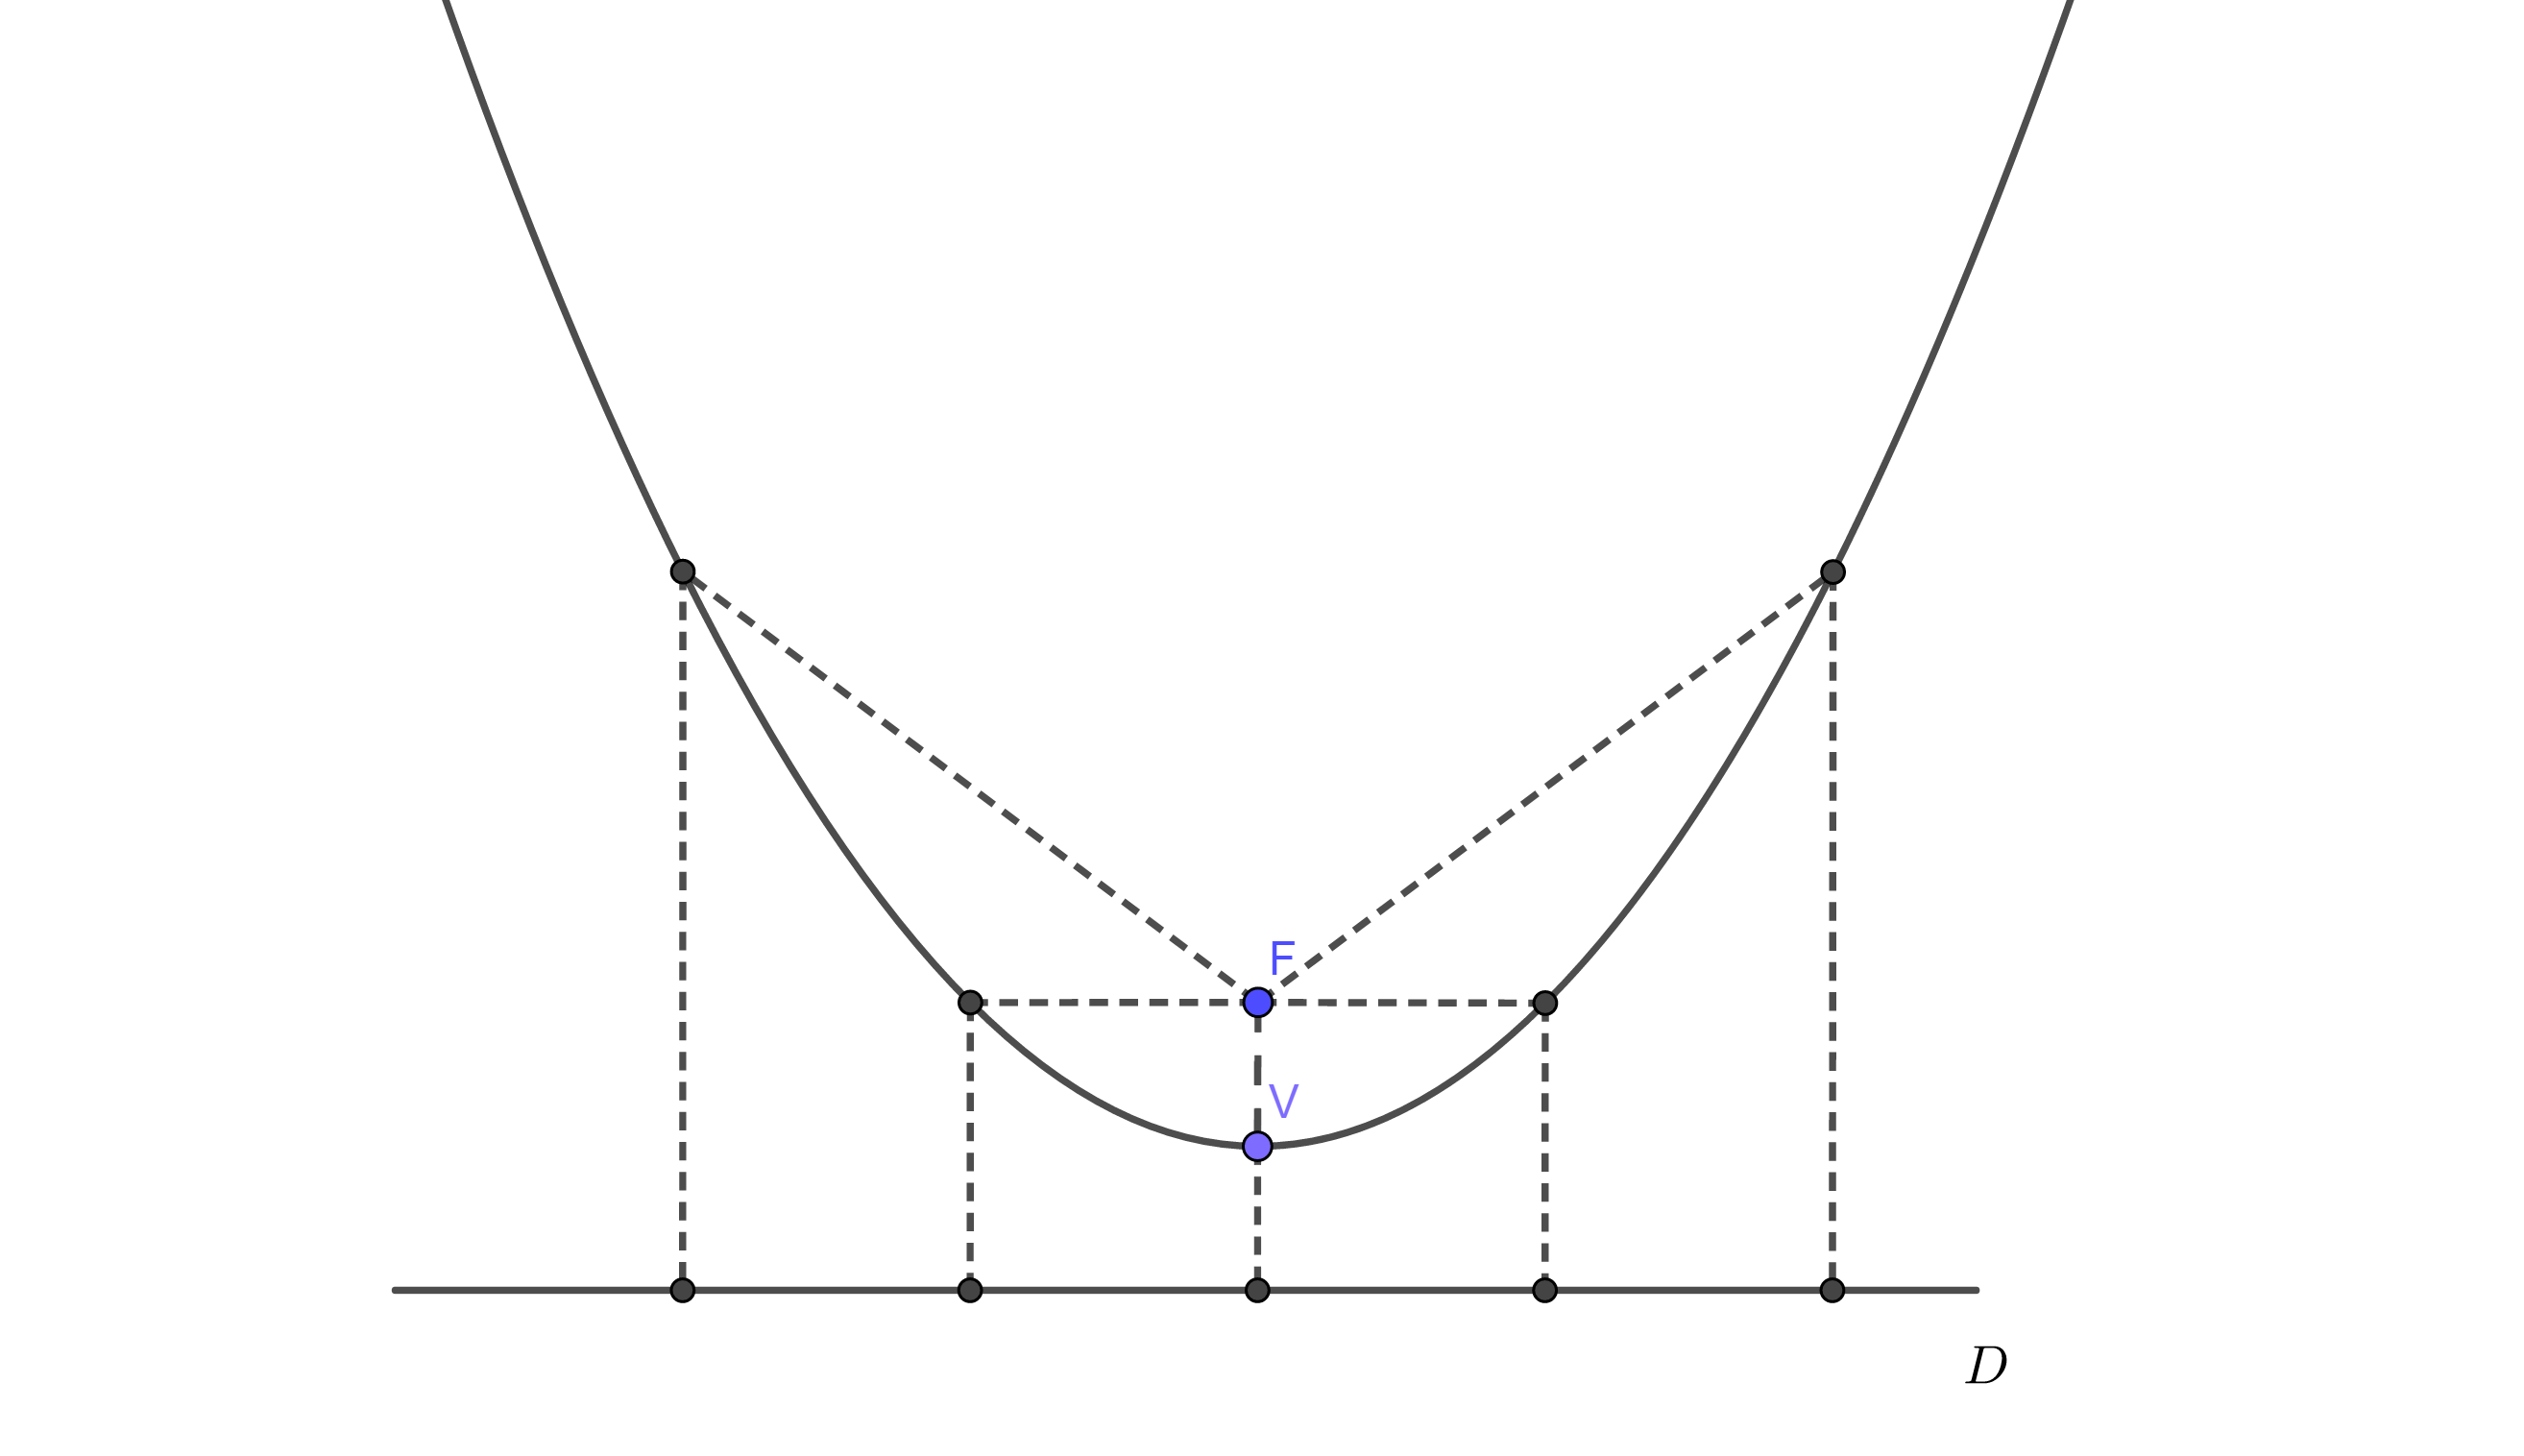
\includegraphics{parabola1.png}
\end{figure}

\begin{defi}[Standard Equation of a Horizontal Parabola]
    The equation with Vertex $V:(h,k)$ and focal length $c$ is
    \begin{equation*}
        (y-h)^2 = \pm4c(x-k)
    \end{equation*}
    Opening either to the right or left.
\end{defi}
\textbf{Parts of Parabola}
\begin{itemize} 
    \item \emph{Vertex} $\rightarrow$ The point midway between the focus and the
    directrix.
    \item \emph{Focus} $\rightarrow$ Fixed point that is $c$ units above or
    below the vertex. (right or left if Horizontal Parabola)
    \item \emph{Directrix} $\rightarrow$ Fixed line that is $c$ units above or
    below the vertex. (right or left if Horizontal Parabola)
    \item \emph{Axis of Symettry}  $\rightarrow$ The line that divides the
    parabola into two parts which are mirror images of each other.
    \item \emph{Latus Rectum}  $\rightarrow$ The line segment through the focus
    perpendicular to the axis of symmetry and whose length is $4c$ called the
    \emph{focal diameter}.
\end{itemize}

\subsection{Ellipse}
\begin{defi}[Ellipse]
     Given two distinct points $F_1$ and $F_2$ in the plane and a fixed distance
     $d$, an \emph{ellipse} is the set of all points $(x,y)$ in the plane such
     that the sum of each of the distances from $F_1$ and $F_2$ to $(x,y)$ is
     $d$. The points $F_1$ and $F_2$ are called the \emph{foci} of the
     \emph{ellipse}.
\end{defi}
\begin{defi}[Standard Equation of a Horizontal Ellipse]
     The standard equation of an ellipse with Center $C:(h,k)$ with the
      \emph{major axis} of length $2a$ along the $x$-axis  and a \emph{minor
      axis} of length $2b$ along the $y$-axis is
      \begin{equation*}
           \dfrac{(x-h)^2}{a^2}+\dfrac{(y-k)^2}{b^2}=1
      \end{equation*}
\end{defi}
\begin{figure}[h]
     \centering
     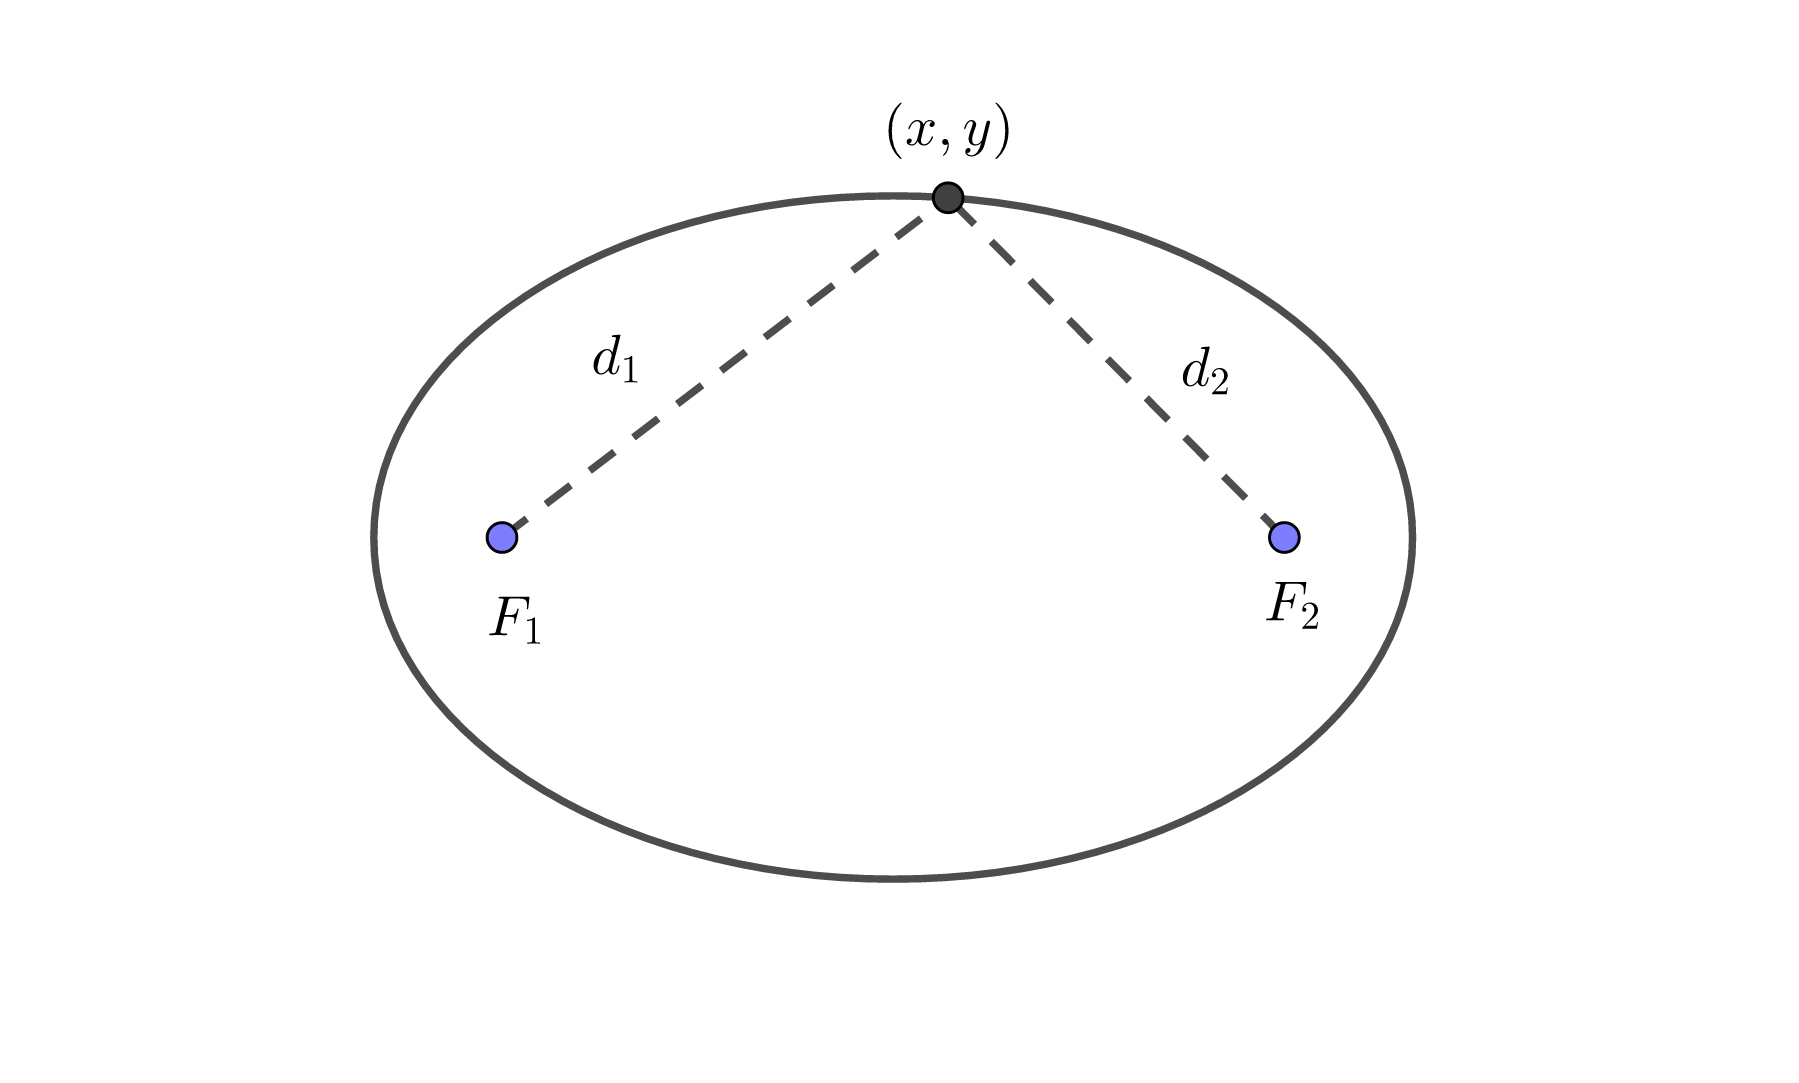
\includegraphics[scale = 2]{ellipse1.png}
\end{figure}
From the definition of an ellipse, defining the foci $F_1:(-c,0)$ and
 $F_2:(c,0)$ and $V:(a,0)$, lying all on the same line, we can conclude the
 following:
\begin{align*}
     \text{distance from $(-c,0)$ to $(a,0)$} + 
     \text{distance from $(c,0)$ to $(a,0)$} &= d \\[1.25ex]
     (a-c) + (a+c) &= d \\[1.25ex]
     2a &= d
\end{align*}
Define the following, the foci are $F_1:(-c,0)$ and $F_2:(c,0)$, and letting a
point on the ellipse be a covertex $P:(b,0)$, from the definition of an ellipse,
we can conclude the following:
\begin{align*}
     \text{distance from $(-c,0)$ to $(0,b)$} + 
     \text{distance from $(c,0)$ to $(0,b)$} &= d \\[1.25ex]
     \sqrt{(-c-0)^2+(0-b)^2} + \sqrt{(c-0)^2+(0-b)^2} &= 2a \\[1.25ex]
     \sqrt{c^2+b^2}+\sqrt{c^2+b^2} &= 2a \\[1.25ex]
     2\sqrt{c^2+b^2} &= 2a \\[1.25ex]
     \sqrt{c^2+b^2} &= a
\end{align*}
From this we get $a^2=b^2+c^2$, or $c^2=a^2-b^2$.
\begin{defi}[Standard Equation of a Vertical Ellipse]
    The standard equation of an ellipse with Center $C:(h,k)$ with the
      \emph{major axis} of length $2a$ along the $y$-axis  and a \emph{minor
      axis} of length $2b$ along the $x$-axis is
      \begin{equation*}
           \dfrac{(x-h)^2}{b^2}+\dfrac{(y-k)^2}{a^2}=1
      \end{equation*}
\end{defi}
\textbf{Parts of Ellipse}
\begin{itemize}
    \item \emph{Center} $\rightarrow$ The intersection of the major and minor
        axis. The midpoint of the line segment joining the foci.
    \item \emph{Foci} $\rightarrow$ Each focus is $c$ units away from the
        center. For any points on the ellipse,  the sum of its distances from
        the focis is $2a$.
    \item \emph{Vertices} $\rightarrow$ Points on the ellipse that are collinear
        with the center and foci. Each vertex is $a$ units away from the center.
        Endpoints of the \emph{major axis}.  
    \item \emph{Covertices} $\rightarrow$ Points on the ellipse that are $b$
        units away from the center. Endpoints of the \emph{minor axis}.
    \item \emph{Directrices} $\rightarrow$ Each \emph{directrix} is parallel to
         the \emph{minor axis} and is located outside the curve. 
        \begin{center}
            \emph{Horizontal Ellipse}: $x=\pm \dfrac{a^2}{c}$ \qquad
            \emph{Vertical Ellipse}: $y=\pm \dfrac{a^2}{c}$
        \end{center}
    \item \emph{Latera Recta} $\rightarrow$ \emph{Latus Rectume} of an ellipse
        is a line segment perpendicular to the major axis through any of the
        foci and whose endpoints lie on the ellipse.
        \begin{center}
             Length of Latus Rectum: $\dfrac{2b^2}{a}$
        \end{center}
    \item \emph{Major Axis} $\rightarrow$ The line segment joining the vertices
        and contains the foci.
        \begin{center}
             Length of Major Axis: $2a$
        \end{center}
    \item \emph{Minor Axis} $\rightarrow$ The line segment joining the
            covertices.
            \begin{center}
                 Length of Minor Axis: $2b$
            \end{center}
    \item \emph{Eccentricity} $\rightarrow$ denoted by $e$ is the ratio
            \begin{equation*}
                 e = \dfrac{\text{Distance from center to foci}}
                 {\text{Distance from center to vertex}} = \dfrac{c}{a}
            \end{equation*}
\end{itemize}
\newpage
\subsection{Hyperbola}
\begin{defi}
    Given two distinct points $F_1$ and $F_2$ in the plane and a fixed distance
    $d$, a hyperbola is the set of all points $(x,y)$ in the plane such that the
    absolute value of the difference of each of the distances from $F_1$ and
    $F_2$ to $(x,y)$ is $d$. The points $F_1$ and $F_2$ are called the foci of
    the hyperbola.
\end{defi}

\begin{figure}[h]
      \centering
      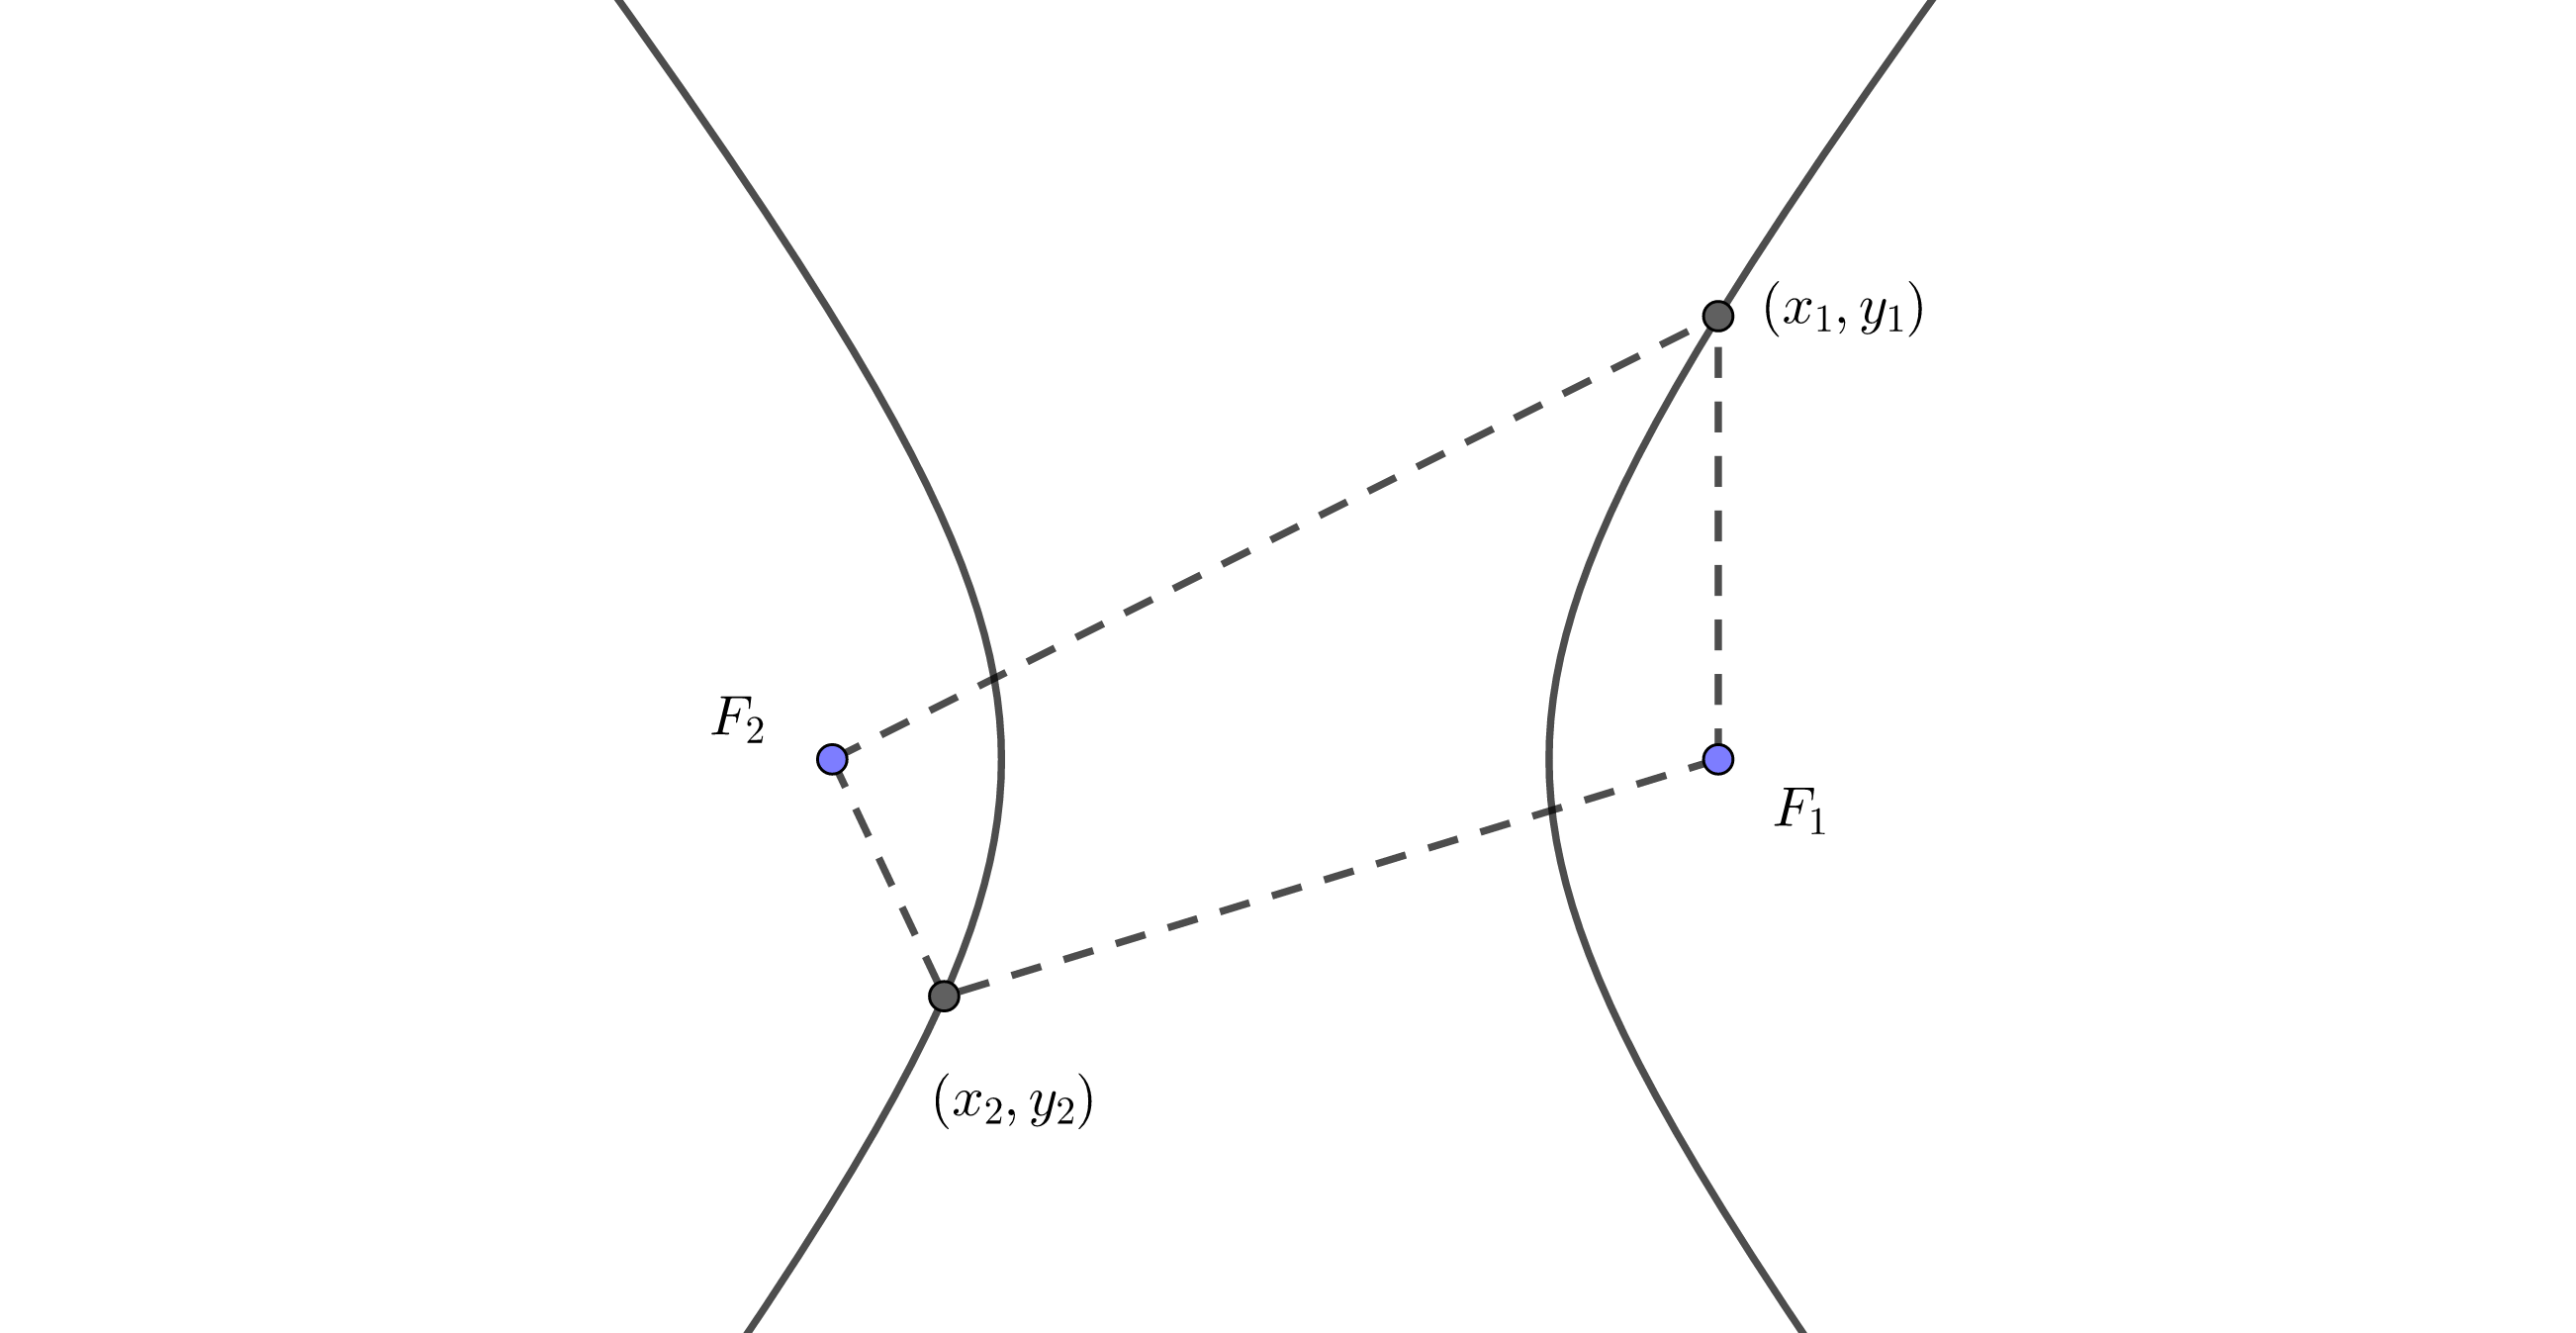
\includegraphics[scale = 1.6]{hyperbola1.png}
\end{figure}

Since $V:(a,0)$ is on the hyperbola, it must satisfy the definition. That is,
the distance from $(-c,0)$ to $(a,0)$ minus the distance from $(c,0)$ to $(a,0)$
must equal the fixed distance $d$. Since all these points lie on the same line,
we get
\begin{align*}
     \left \lvert \text{distance from $(-c,0)$ to $(a,0)$} -
     \text{distance from $(c,0)$ to $(a,0)$} \right \rvert &= d \\[1.25ex]
     \left \lvert (a+c) - (c-a) \right \rvert &= d \\[1.25ex]
     \left \lvert 2a \right \rvert &= d \\[1.25ex]
     2a &= d 
\end{align*}
We also have the following equation
\begin{equation*}
      c^2 = a^2 + b^2
\end{equation*}
\begin{defi}[Standard Equation of a Horizontal Hyperbola]
      For positive numbers $a$ and $b$, the equation of a horizontal hyperbola
       with center $(h,k)$ is:
       \begin{equation*}
             \dfrac{(x-h)^2}{a^2}+\dfrac{(y-k)^2}{b^2} = 1
       \end{equation*}
       A hyperbola with branches that opens to the left and right.
\end{defi}
If the roles of $x$ and $y$ were interchanged, then the hyperbola’s branches
would open upwards and downwards and we would get a 
\emph{Vertical Hyperbola}
\begin{defi}[Standard Equation of a Vertical Hyperbola]
     For positive numbers $a$ and $b$, the equation of a horizontal hyperbola
     with center $(h,k)$ is:
     \begin{equation*}
          \dfrac{(y-h)^2}{a^2}+\dfrac{(x-k)^2}{b^2} = 1
     \end{equation*}
\end{defi}
\textbf{Parts of Hyperbola}
\begin{itemize}
     \item \emph{Transverse Axis} $\rightarrow$ The equivalent of the major axis
          of an ellipse. It contains the foci, center, and vertices as its
          endpoints.
     \item \emph{Conjugate Axis} $\rightarrow$ The equivalent of the minor axis
     of an ellipse. The line segment which is a perpendicular bisector of the
     transverse axis.
     \item \emph{Latera Recta} $\rightarrow$ A line segment that contains the
     foci and perpendicular to the transverse axis.
          \begin{center}
                Length of Latus a Rectum: $\dfrac{2b^2}{a}$
          \end{center}
     \item \emph{Directrices} $\rightarrow$ A directrix is parallel to the
     conjugate axis.
          \begin{center}
                Distance from center: $\dfrac{a^2}{c}$
          \end{center}
     \item \emph{Asymptotes} $\rightarrow$ Two lines passing through the center
     with each branch of the hyperbola approaching the asymptotes  as $|x|
     \rightarrow \infty$.
          \begin{center}
                Equation of Asymptotes: $y= \pm \dfrac{b}{a}x$
          \end{center}
\end{itemize}

\newpage
\subsection{Applications of Parabola}

\begin{eg}
     The cable of a suspension bridge hangs in the shape of a parabola. The
     towers supporting the cable are $400$ ft apart and $150$ ft high. If the
     cable, at its lowest, is $30$ ft above the bridge at its midpoint, how high
     is the cable $50$ ft away (horizontally) from either tower?
     \medbreak
     \begin{proof}
           We may write it with the equation $(x-0)^2=a(y-30)$; since we dont
          need the focal distance,we use the simpler variable $a$ in place of
          $4c$. Since the towers are $150$ ft high and $400$ ft apart, we deduce
          that $(200,150)$ is a point on the parabola.
          \begin{align*}
                x^2 &= a(y-30) \\[1.25ex]
                (200)^2 &= a(150-30) \\[1.25ex]
                a &= \dfrac{200^2}{120} = \dfrac{1000}{3}
          \end{align*}
          The parabola has equation $x^2=\dfrac{1000}{3}(y-30)$ or equivalently,
          $y=0.003x^2+30$. For the two points on the parabola $50$ ft away from
          the towers, $x=150$ or $x=-150$. If $x =150$, then
          \begin{equation*}
                y = 0.0003(150)^2 +30 = 97.5.
          \end{equation*} 
          Thus the cable is $97.5$ ft high $50$ ft away from the tower.
     \end{proof}
\end{eg}
\begin{eg}
      A satellite dish has a hape calleda paraboloid, where each cross-section
      is a parabola. Since radio signals (parallel to the axis) will bounce off
      the surface of the dish to the focus, the receiver should be placed at the
      focus. How far should the receiver be from the vertex, if the dish is $12$
      ft across and $4.5$ ft deep at the vertex?
      \begin{proof}
            We take a cross-section of the satellite dish drawn on a rectungular
            coordinate system, with the vertex at the origin. From the problem,
            we deduce that $(6,4.5)$ is a point on the parabola. We need the
            distance of the focus from the vertex, i.e, the value of $c$ in
            $x^2=4cy$.
            \begin{align*}
                 x^2 &= 4cy \\[1.25ex]
                 6^2 &= 4c(4.5) \\[1.25ex]
                 c &= \dfrac{36}{4 \cdot 4.5} = 2
            \end{align*}
            Thus, the receiver should be $2$ ft away from the vertex. 
      \end{proof} 
\end{eg}

\newpage
\subsection{Applicatios of Hyperbola}
\begin{eg}
      An explosion is recorded by two microphones that are $10$km apart. 
      the first microphone receives the sound $3$ seconds before the second 
      microphone. Assuming the sound travels at $1.2$ km/s, determing the
     possible locations of the expolosion relative to the location of the 
      microphone.
     \begin{proof}
           Let $M_A$ be the first microphone and $M_B$ the second microphone
           which are the foci the hyperbola. Let the explosion be at the point
           $:V:(a,0)$. It is given that $M_A$ received the sound $3$ seconds
           before $M_B$ given that sound travels at $1.2$ km/s, we can solve for
           the distance between the two vertices.
          \begin{align*}
               3 \cdot 1.2 &= 3.6\;km = 2a \\[1.25ex]
               a &= 1.8 \\[1.25ex]
               a^2 &= 3.24
          \end{align*}
          We can assume that the hyperbola is of the form 
          \begin{equation*}
               \dfrac{x^2}{a^2}-\dfrac{y^2}{b^2}=1
          \end{equation*}
          We know that the distance between $M_A$ and $M_B$ is $10$ km which
          serves as  the focal distance $2c$.
          \begin{align*}
               2c &= 10 \\[1.25ex]
               c &= 5 \\[1.25ex]
               c^2 &= 25
          \end{align*}
          Using $c^2=a^2+b^2$ we get 
          \begin{align*}
               c^2&=a^2+b^2 \\[1.25ex]
               b^2 &= c^2-a^2 \\[1.25ex]
               b^2 &= 25-3.24 \\[1.25ex]
               b^2 &= 21.76
          \end{align*}
          The equation of the hyperbola with microphones at each focus is 
          \begin{equation*}
               \dfrac{x^2}{3.24}-\dfrac{y^2}{21.76}=1
          \end{equation*}
          If we assume that $M_A$ resides at the right side, then the explosion
          occured on the right branch of the hyperbola, which is closer to
          $M_A$.
     \end{proof}
\end{eg}

\newpage
\section{Linear Systems of Equations}
We will discuss Linear Algebra instead of basic Linear equations. Topics
such as matrices, pivots, gaussian elimination, spans, linear combinations,
 vector spaces, and linear transformations
\subsection{Linear Equations}
\begin{defi}[Linear Equations]
      A \emph{linear equation} is an equation that may be put in the form 
      \begin{equation*}
           a_1x_1+\cdots+a_nx_n+b=0
      \end{equation*}
      where $x_1, \ldots ,x_n$ are the variables, and $b,a_1,\ldots,a_n$ are the
      coefficients. (where often it is the case that $x_i \in \mathbb{R} $ ).
\end{defi}
We can solve system of linear equations for example in $\mathbb{R}^2$ where
there are only two variables.
\begin{eg}
      If we graph the two lines 
      \begin{align*}
           3x+2y&=4 \\[1.25ex]
           6x+47 &= 5
      \end{align*}
      we can see that they are parallel and do not intersect, so that 
      this system of linear equations has no solution.
\end{eg}
\begin{eg}
     If we graph the two lines 
     \begin{align*}
          3x+2y&=5 \\[1.25ex]
          x+y &= 2
     \end{align*}
     it is easy to see that the two lines are not parallel and intersect at the
point $(1, 1)$, so that this system of two linear equations has exactly one
solution.
\end{eg}
\begin{eg}
     If we graph the two lines 
     \begin{align*}
          3x+2y &=5 \\[1.25ex]
          6x+4y &=10
     \end{align*}
     It is easy to see that the two lines overlap completely, so that this
system of two linear equations has infinitely many solutions.
\end{eg}
In general, we shall study a system of $m$ linear equations of the form
\begin{align*}
     a_{11}x_1 + a_{12}x_2 + \cdots + a_{1n}x_n &= d_1\\
     a_{21}x_1 + a_{22}x_2 + \cdots + a_{2n}x_n &= d_2\\
     \vdots&\\
     a_{m1}x_1 + a_{m2}x_2 + \cdots + a_{mn}x_n &= d_m
   \end{align*}
with $n$ variables $x_1,x_2,\cdots,x_n$. Here we may not be so lucky as to be
able to see geometrically what is going on. We therefore need to study the
problem from a more algebraic viewpoint.

We can omit the variables, then the system can be represented by 
an array of all the coefficients known as the \emph{augmented matrix}.
\begin{equation*}
     \begin{pmatrix}
          a_{11} & a_{12} & \ldots & a_{1n} &\bigm| & b_1 \\
          a_{21} & a_{22} & \ldots & a_{2n} &\bigm| & b_2 \\
          \vdots & \vdots &        & \vdots &\bigm| & b_3 \\ 
          a_{m1} & a_{m2} & \ldots & a_{mn} &\bigm| & b_4
      \end{pmatrix}
\end{equation*}
We can also write it as $A\mathrm{\textbf{x}}=\mathrm{\textbf{b}}$, 
a matrix $A$ multiplied by the vector $\mathrm{\textbf{x}}$ is the 
vector $\mathrm{\textbf{b}}$, where
\begin{equation*}
     A =
     \begin{pmatrix}
          a_{11} & a_{12} & \ldots & a_{1n}   \\
          a_{21} & a_{22} & \ldots & a_{2n}  \\
          \vdots & \vdots &        & \vdots  \\ 
          a_{m1} & a_{m2} & \ldots & a_{mn} 
      \end{pmatrix}
\end{equation*}
and
\begin{equation*}
      \mathrm{\textbf{b}} =
     \begin{pmatrix}
          b_{1}   \\
          b_{2}    \\
          \vdots    \\ 
          b_{m}   
      \end{pmatrix}
\end{equation*}
represents the coefficients and
\begin{equation*}
     \mathrm{\textbf{x}} =
    \begin{pmatrix}
         x_{1}   \\
         x_{2}    \\
         \vdots    \\ 
         x_{m}   
     \end{pmatrix}
\end{equation*}

represents the variables.
\begin{eg}
     The array
     \begin{equation*}
          \begin{pmatrix}
               1 & 3 & 1 & 5 & 1 &\bigm|  5\; \\
               0 & 1 & 1 & 2 & 1 &\bigm|  4\; \\ 
               2 & 4 & 0 & 7 & 1 &\bigm|  3\;
           \end{pmatrix}
     \end{equation*}
     represents the three linear equations
     \begin{align*}
          x_1+3x_2+x_3+5x_4+x_5 &= 5, \\
               x_2+x_3+2x_4+x_5 &= 4, \\
          2x_1+4x_2+  +7x_4+x_5 &= 3, \\
     \end{align*}
     with five variables $x_1,x_2,x_3,x_4,x_5$. We can also write
     \begin{equation*}
          \begin{pmatrix}
               1 & 3 & 1 & 5 & 1  \; \\
               0 & 1 & 1 & 2 & 1  \; \\ 
               2 & 4 & 0 & 7 & 1  \;
           \end{pmatrix}
           \begin{pmatrix}
               x_{1} \\
               x_{2} \\
               x_{3} \\ 
               x_{4} \\ 
               x_{5}
           \end{pmatrix} =
           \begin{pmatrix}
               5 \\
               4 \\
               3
           \end{pmatrix}
     \end{equation*}
\end{eg}


\subsection{Elementary Row Operations}

\begin{prop}[Elementary Row Operations]
     There are three types of elementary matrices, which correspond to three
     types of row operations
      \begin{enumerate}
          \item \textbf{Row Switching} $\rightarrow$ A row within the matrix can be
          switched with another row.
             \begin{equation*}
                  R_i \leftrightarrow R_j
             \end{equation*}
          \item \textbf{Row Multiplication} $\rightarrow$ Each element in a row
          can be multiplied by a non-zero constant.
          \begin{equation*}
               kR_i \rightarrow R_i \text{, where $k \neq 0$}
          \end{equation*}
          \item \textbf{Row Addition} $\rightarrow$ A row can be replaced by the
          sum of that row and a multiple of another row.
          \begin{equation*}
               R_i + kR_j \rightarrow R_i \text{, where $i \neq j$}
          \end{equation*}
      \end{enumerate}
\end{prop}
\begin{eg}
      Consider again the system of linear equations
      \begin{align*}
          x_1+3x_2+x_3+5x_4+x_5 &= 5, \\
               x_2+x_3+2x_4+x_5 &= 4, \\
          2x_1+4x_2+  +7x_4+x_5 &= 3, \\
     \end{align*}
     represented by the array
     \begin{equation*}
          \begin{pmatrix}
               1 & 3 & 1 & 5 & 1 &\bigm|  5\; \\
               0 & 1 & 1 & 2 & 1 &\bigm|  4\; \\ 
               2 & 4 & 0 & 7 & 1 &\bigm|  3\;
           \end{pmatrix}
     \end{equation*}
\begin{proof}
     Let us now perform elementary row operations on the augmented matrix. 
     We first label the rows as $R_1, R_2,\:and\;R_3$.

     Adding $-2$ times the first row to the third row.
     \begin{equation*}
          -2R_1 + R_3 \rightarrow R_3 \qquad
          \begin{pmatrix}
               1 & 3 & 1 & 5 & 1 &\bigm|  5\; \\
               0 & 1 & 1 & 2 & 1 &\bigm|  4\; \\ 
               0 & -2 & -2 & -3 & -1 &\;\bigm|  -7 \;
           \end{pmatrix}
     \end{equation*}
     From here, we add $2$ times the second row to the third row to obtain
     \begin{equation*}
          2R_2 + R_3 \rightarrow R_3 \qquad
          \begin{pmatrix}
               1 & 3 & 1 & 5 & 1 &\bigm|  5\; \\
               0 & 1 & 1 & 2 & 1 &\bigm|  4\; \\ 
               0 & 0 & 0 & 1 & 1 &\;\bigm|  1 \;
          \end{pmatrix}
     \end{equation*}
     Next, we add $-3$ times the second row to the first row to obtain.
     \begin{equation*}
          -3R_2 + R_1 \rightarrow R_3 \qquad
          \begin{pmatrix}
               1 & 0 & -2 & -1 & -2 &\bigm|  -7\; \\
               0 & 1 & 1 & 2 & 1 &\bigm|  4\; \\ 
               0 & 0 & 0 & 1 & 1 &\;\bigm|  1 \;
          \end{pmatrix}
     \end{equation*}
     Next, we add the third row to the first row to obtain
     \begin{equation*}
          3R_3 + R_1 \rightarrow R_3 \qquad
          \begin{pmatrix}
               1 & 0 & -2 & 0 & -1 &\bigm|  -6\; \\
               0 & 1 & 1 & 2 & 1 &\bigm|  4\; \\ 
               0 & 0 & 0 & 1 & 1 &\;\bigm|  1 \;
          \end{pmatrix}
     \end{equation*}
     Finally, we add $-2$ times the third row to the second row to obtain
     \begin{equation*}
          -2R_3 + R_2 \rightarrow R_3 \qquad
          \begin{pmatrix}
               1 & 0 & -2 & 0 & -1 &\bigm|  -6\; \\
               0 & 1 & 1 & 0 & -1 &\bigm|  2\; \\ 
               0 & 0 & 0 & 1 & 1 &\;\bigm|  1 \;
          \end{pmatrix}
     \end{equation*}
     We know that this augmented matrix is equivalent to the 
     system of linear equations:
     \begin{align*}
          x_1+   -2x_3+   -x_5 &= -6, \\
               x_2+x_3+   -x_5 &= 2, \\
                       x_4+x_5 &= 1, 
     \end{align*}
     First of all, take the third equation 
     \begin{equation*}
          x_4+x_5 =1
     \end{equation*}
     If we let $x_5 = t$, then $x_4=1-t$. Substituting to the 
     second equation, we obtain
     \begin{equation*}
          x_2+x_3 =2+t
     \end{equation*}
     If we let $x_3=s$, then $x_2=2+t-s$. Substituting all these
     info into the first equation, we obtaion
     \begin{equation*}
          x_1 =-6+t+2s
     \end{equation*}
     Hence
     \begin{equation*}
          \mathrm{\textbf{x}}=(x_1,x_2,x_3,x_4,x_5) = (-6+t+2s,2+t-s,s,1-t,t)
     \end{equation*}
     is a solution of the system of linear equations for every 
     $s,t \in \mathbb{R}$.
\end{proof}
\end{eg}
dwadacwad
\end{document}